No contexto deste trabalho, o problema da colorização de uma imagem será abordado como uma \emph{tarefa de regressão}, cujo objetivo é obter uma estimativa dos parâmetros de coloração dos pixels. De maneira mais detalhada, a Figura \ref{fig:aprendizado} ilustra o conjunto de passos a ser realizado.

\begin{figure}[h]
	\centering
	\caption{Detalhamento do processo de aprendizado.}
	\label{fig:aprendizado}
	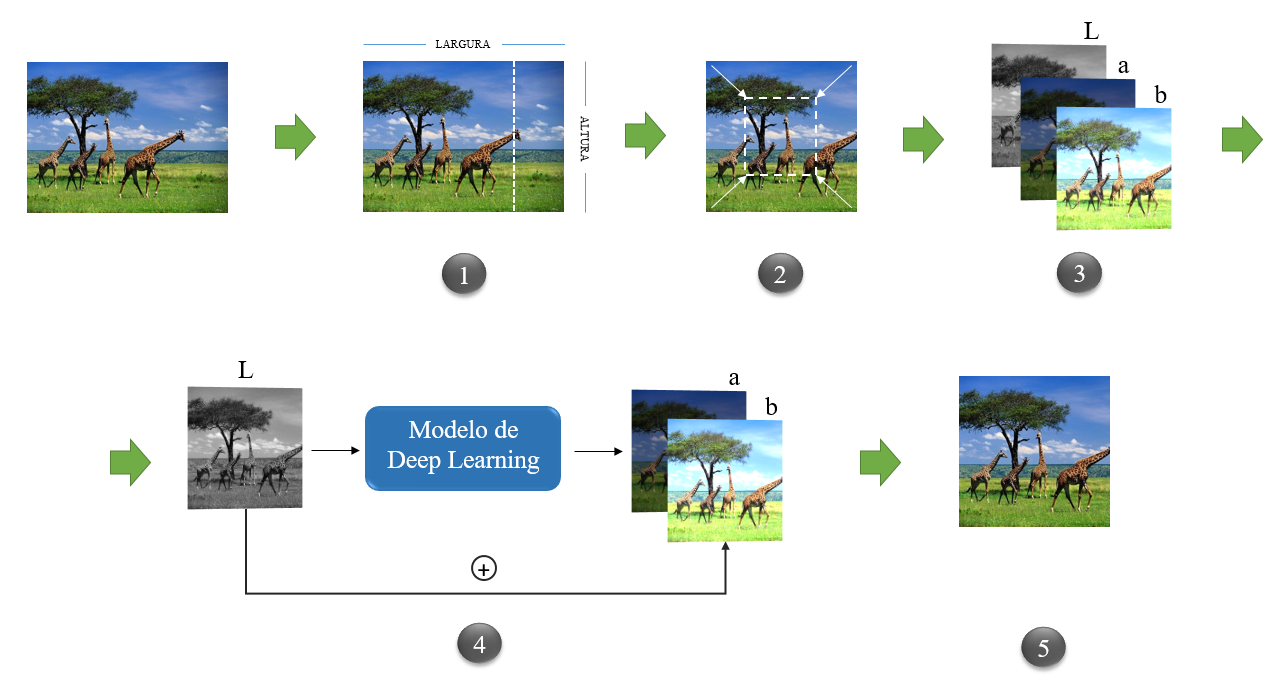
\includegraphics[width=0.95\textwidth]{./img/aprendizado}
\end{figure}

Dada uma imagem em tons de cinza que se deseja colorir, o primeiro passo a ser realizado (Passo 1) consiste no redimensionamento da imagem de acordo com a dimensão predominante (altura ou largura), com vistas a obter uma imagem quadrada. Em seguida, para que seja fornecida como entrada para os modelos de DL, a imagem será redimensionada para $128 \times 128$ pixels (Passo 2). Após esta etapa, o espaço de cores da imagem será convertido de RGB para CIELab (Passo 3). Desta conversão, o parâmetro de luminosidade $L$ será fornecido para o modelo de DL, cujo objetivo será produzir duas matrizes com os valores de coloração $a$ e $b$ (Passo 4). Por fim, a luminosidade $L$, já conhecida, será combinada com as matrizes de coloração $a$ e $b$ produzidas, compondo uma versão colorida da imagem inicial (Passo 5).

Para que os modelos propostos para realização da coloração produzam resultados factíveis, é necessária uma etapa de treinamento, em que imagens coloridas serão fornecidas sucessivamente às redes para ajustes dos pesos, produzindo mapas de características mais fidedignos ao domínio do problema. A base de dados a ser utilizada para esta etapa será descrita na seção a seguir.

No escopo deste trabalho serão consideradas as arquiteturas canônicas de CNNs VGGNet  e ResNet as quais serão ajustadas ao problema em questão mediante TL. Diferentes valores de parâmetros e hiperparâmetros (épocas, taxa de aprendizado, \emph{batch size}, etc.) serão considerados, sempre que possível, buscando um melhor ajuste do modelo ao problema em questão.

Nesta tarefa de regressão, realizada de acordo com o paradigma supervisionado, a métrica de desempenho utilizada será o Erro Quadrático Médio (MSE, do inglês \emph{Mean Squared Error}), definido como:

\begin{equation}
\textrm{MSE} = \frac{1}{n}\sum_{i=1}^n (y_i - \hat{y}_i)^{2}, \label{eq:mse}
\end{equation} em que $y_i$ é o valor real esperado para o exemplo $i$, $\hat{y}_i$ é o valor previsto pelo modelo para este exemplo e $n$ é o número de amostras presentes no conjunto de dados \cite{ref:faceli}.

O treinamento e testes das CNNs seguirão a abordagem \emph{Holdout} de validação cruzada, em que $70\%$ dos dados serão utilizados no treino e ajuste de parâmetros e o restante para avaliação, com vista a capturar a qualidade da generalização proposta pelos modelos considerados \cite{ref:brink}.
